\documentclass[11pt,a4paper]{article}
			\usepackage[french]{babel}
					
				\usepackage{pifont}  
				\usepackage[utf8x]{inputenc}
				\usepackage[T1]{fontenc} 
				\usepackage{lmodern}			
				\usepackage{fancyhdr}
				\usepackage{textcomp}
				\usepackage{makeidx}
				\usepackage{tabularx}
				\usepackage{multicol}
				\usepackage{multirow}
				\usepackage{longtable}
				\usepackage{color}
				\usepackage{soul}
				\usepackage{boxedminipage}
				\usepackage{shadow}
				\usepackage{framed}			
				\usepackage{array}
				\usepackage{url}
				\usepackage{ragged2e}
				\usepackage{fancybox}
				\newcommand{\cadretitre}[2]{
				  \vspace*{0.8\baselineskip}
				  \begin{center}%
				  \boxput*(0,1){%
					%\colorbox{white}{\Large\textbf{\ #1\ }}%
				  }%
				  {%
					\setlength{\fboxsep}{10pt}%
				    \Ovalbox{\begin{minipage}{.8\linewidth}\begin{center}\Large\sffamily{#2}\end{center}\end{minipage}}}%
				  \end{center}
				  \vspace*{2\baselineskip}
				  }
			
			\makeatletter
			\def\@seccntformat#1{\protect\makebox[0pt][r]{\csname the#1\endcsname\quad}}
			\makeatother

				% Permet d'afficher qqchose à une positin absolue
				\usepackage[absolute]{textpos}
				\setlength{\TPHorizModule}{1cm}
				\setlength{\TPVertModule}{\TPHorizModule}
	
				\usepackage[titles]{tocloft}
				\setlength{\cftbeforesecskip}{0.5ex}
				\setlength{\cftbeforesubsecskip}{0.2ex}
				\addto\captionsfrench{\renewcommand\contentsname{}}
				
				\usepackage[font=scriptsize]{caption}
				
				\usepackage{listings}
\lstdefinestyle{lstverb}
  {
    basicstyle=\footnotesize,
    frameround=tttt, frame=trbl, framerule=0pt, rulecolor=\color{gray},
    lineskip=-1pt,   % pour rapprocher les lignes
    flexiblecolumns, escapechar=\\,
    tabsize=4, extendedchars=true
  }
\lstnewenvironment{Java}[1][]{\lstset{style=lstverb,language=java,#1}}{}
				\ifx\pdfoutput\undefined
					\usepackage{graphicx}
				\else
					\usepackage[pdftex]{graphicx}
				\fi
				\usepackage[a4paper, hyperfigures=true, colorlinks, linkcolor=black, citecolor=blue,urlcolor=blue, pagebackref=true, bookmarks=true, bookmarksopen=true,bookmarksnumbered=true,
                pdfauthor={}, pdftitle={TD Boucles}, pdfkeywords={TD Boucles, },pdfpagemode=UseOutlines,pdfpagetransition=Dissolve,nesting=true,
				backref, pdffitwindow=true, bookmarksnumbered=true]{hyperref}
				\usepackage{supertabular}
				\usepackage[table]{xcolor}
				\usepackage{url}
				\usepackage{caption} 
				\setlength{\parskip}{1.3ex plus 0.2ex minus 0.2ex}
				\setlength{\parindent}{0pt}
				
				\makeatletter
				\def\url@leostyle{ \@ifundefined{selectfont}{\def\UrlFont{\sf}}{\def\UrlFont{\footnotesize\ttfamily}}}
				\makeatother
				\urlstyle{leo}
				
				\definecolor{examplecolor}{rgb}{0.156,0.333,0.443}
				\definecolor{definitioncolor}{rgb}{0.709,0.784,0.454}
				\definecolor{exercisecolor}{rgb}{0.49,0.639,0}
				\definecolor{hintcolor}{rgb}{0.941,0.674,0.196}
				\definecolor{tableHeadercolor}{rgb}{0.709,0.784,0.454}
				\definecolor{tablerowAltcolor}{rgb}{.866,.905,.737}
				\definecolor{tablerowAlt2color}{rgb}{.968,.976,.933}
				\definecolor{verylightgray}{rgb}{0.98,0.98,0.98}
				
				\newenvironment{fshaded}{
				\def\FrameCommand{\fcolorbox{framecolor}{shadecolor}}
				\MakeFramed {\FrameRestore}}
				{\endMakeFramed}
				
				\newenvironment{fexample}[1][]{\definecolor{shadecolor}{rgb}{.913,.913,.913}
				\definecolor{framecolor}{rgb}{.156,.333,.443}
				\begin{fshaded}}{\end{fshaded}} 
				
				\newenvironment{fdefinition}{\definecolor{shadecolor}{rgb}{.913,.913,.913}
				\definecolor{framecolor}{rgb}{.709,.784,.454}
				\begin{fshaded}}{\end{fshaded}}
				
				\newenvironment{fexercise}{\definecolor{shadecolor}{rgb}{.913,.913,.913}
				\definecolor{framecolor}{rgb}{.49,.639,0}
				\begin{fshaded}}{\end{fshaded}}
				
				\newenvironment{fhint}{\definecolor{shadecolor}{rgb}{.913,.913,.913}
				\definecolor{framecolor}{rgb}{.941,.674,.196}
				\begin{fshaded}}{\end{fshaded}}	
				
				\newcommand{\PreserveBackslash}[1]{
				\let\temp=\\#1\let\\=\temp
				}
				\let\PBS=\PreserveBackslash
				\newcolumntype{A}{>{\PBS\raggedright\small\hspace{0pt}}X}
				\newcolumntype{L}[1]{>{\PBS\raggedright\small\hspace{0pt}}p{#1}}
				\newcolumntype{R}[1]{>{\PBS\raggedleft\small\hspace{0pt}}p{#1}}
				\newcolumntype{C}[1]{>{\PBS\centering\small\hspace{0pt}}p{#1}}
				
				\makeindex
				
				\title{TD Boucles}	
			\date{}
			\author{\scriptsize{}}
			\definecolor{light-gray}{gray}{0.8}
			\renewcommand{\headrulewidth}{0pt}
			\fancyhead[L]{
				\footnotesize\textsc{Haute \'Ecole de Bruxelles}\\
	    			\footnotesize\textsc{\'Ecole Sup\'erieure d'Informatique}
			}
			\fancyhead[R]{
				\footnotesize{Bachelor en Informatique}\\
				\footnotesize{Laboratoires Java} - 
			\footnotesize{1\`ere ann\'ee}}
				\fancyfoot[L]{ }
				\fancyfoot[C]{}
				\fancyfoot[R]{\scriptsize{\textcolor{gray}{version 2014-2015 (\today)}}}
				\pagestyle{plain}
				\reversemarginpar
				\usepackage{rotating}						
				\begin{document}
					\begin{textblock}{9}(2,3.2)
						
\includegraphics[width=2cm]{../../../_templates/java/icons/logo-esi}
					\end{textblock}
				
				
				
				
				%\maketitle
				\cadretitre{TD1}{TD Boucles}
				\thispagestyle{fancy}
        \marginpar{\begin{sideways}
            \begin{minipage}[t]{1cm}
            \begin{tiny}
            
\includegraphics[width=1\linewidth,height=1\textheight,keepaspectratio=true]{../../../_templates/java/icons/cc-gris.jpg}
			\end{tiny}
			\end{minipage}
            \begin{minipage}[b]{19cm}
            \begin{tiny}
            \textcolor{gray}{Distribué sous licence Creative Commons Paternité - Partage à l'Identique 2.0 Belgique 
            (\texttt{http://creativecommons.org/licenses/by-sa/2.0/be/})
			\vspace{-1em}
			\\Les autorisations au-delà du champ de cette licence peuvent être obtenues à 
			\texttt{http://www.heb.be/esi}
			- \texttt{mcodutti@heb.be}
			}\end{tiny}
			\end{minipage}
        \end{sideways}}
            \begin{abstract}
			Voyons ici comment incorporer des boucles, les structures r\'ep\'etitives, dans nos codes et comment les utiliser \`a bon escient.
    
            \par
        \end{abstract}
				\vspace{-2em}\tableofcontents
				\pagestyle{plain}
            \clearpage
            \fancyhead[L,C,R]{}
            \fancyfoot[L,C]{}
            \fancyfoot[R]{ \scriptsize{\textcolor{gray}{
				TDBoucle - page \thepage}}}
				\thispagestyle{fancy}
				\pagestyle{fancy}
	   
            \section{Les boucles}
        Si on veut faire effectuer un travail r\'ep\'etitif, il faut indiquer deux choses :
        
					\begin{enumerate}
				
			\item Le travail \`a r\'ep\'eter
			\item La mani\`ere de continuer la r\'ep\'etition ou de l'arr\^eter.
					\end{enumerate}
				
            \par
        \subsection{tant que}
        Le \guillemotleft  \verb@tant que@ \guillemotright  est une structure 
        qui demande \`a l'ex\'ecutant de r\'ep\'eter une t\^ache (une ou
        plusieurs instructions) tant qu'une condition donn\'ee est vraie.
      
            \par
        En pseudo-code :
            \par
        \begin{verbatim}
tant que condition faire
    séquence d’instructions à exécuter
fin tant que
      \end{verbatim}
        La \textbf{condition} est une expression d\'elivrant un r\'esultat 
        \textbf{bool\'een} (vrai ou faux).
      
            \par
        
        Il faut qu'il y ait dans la s\'equence d'instructions comprise entre \verb@tant que@
        et \verb@fin tant que@ au moins \textbf{une instruction qui 
        modifie} une des composantes de \textbf{la condition}
        de telle mani\`ere qu'elle puisse \textbf{devenir fausse} \`a un moment donn\'e. Dans le cas contraire,
        la condition reste \textbf{ind\'efiniment vrai}e et la boucle va tourner sans fin, c'est ce qu'on appelle
        une \textbf{boucle infinie}.
      
            \par
        
        Si la condition est fausse d\`es le d\'ebut, la t\^ache n'est jamais ex\'ecut\'ee.
      
            \par
        \begin{figure}[hbt]
				    \begin{center}
					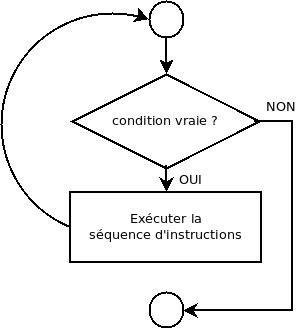
\includegraphics[width=0.8\linewidth,height=0.8\textheight,keepaspectratio=true]{/home/clr/Documents/Cours/DEV1Q2/TDBoucle/fr/image/boucleTq.jpg}
						\end{center}
                
                    \caption[boucleTq.jpg]{boucleTq.jpg}
                \end{figure}
                    
            \par
        Par exemple : 
            \par
        
			
		\subparagraph{Afficher les nombres plus petits que 10} 
		
					\textcolor{white}{.} \par
				On affiche uniquement les nombres inf\'erieurs (pas strictement) \`a 10 .
            \par
        \begin{verbatim}
// Affiche les nombres de 1 à 10.
module compterJusque10 () // version avec tant que
    nb : entier
    nb ← 1 // c’est le premier nombre à afficher
    tant que nb ≤ 10 faire // c’est le premier nombre à afficher
      afficher nb  // on affiche la valeur de la variable nb
      nb ← nb + 1 // on passe au nombre suivant
    fin tant que
fin module
      \end{verbatim}
			
		\subparagraph{Somme de nombres} 
		
					\textcolor{white}{.} \par
				 Apr\`es chaque nombre, on demande \`a l'utilisateur s'il y a encore un nombre \`a additionner.
            \par
        \begin{verbatim}
// Lit des valeurs entières et retourne la somme des valeurs lues.
module sommeNombres() → entier
    valeur : entier // un des termes de l’addition
    somme : entier // la somme
    somme ← 0
    lire valeur
    tant que valeur ≥ 0 faire
      somme ← somme + valeur
      lire valeur // remarquer l’endroit où on lit une valeur.
    fin tant que
retourner somme
fin module
      \end{verbatim}\subsection{faire - jusqu'\`a ce que}
        Cette structure est tr\`es proche du \guillemotleft  \verb@tant que@ \guillemotright  \`a deux diff\'erences pr\`es :
        
					\begin{enumerate}
				
			\item 
            Le \textbf{test} est fait \textbf{\`a la fin} et pas au d\'ebut. 
            La t\^ache est donc toujours \textbf{ex\'ecut\'ee au moins une fois}.
          
			\item On donne la \textbf{condition pour arr\^eter} et pas pour continuer.
					\end{enumerate}
				
            \par
        En pseudo-code :
            \par
        \begin{verbatim}
faire
    séquence d’instructions à exécuter
jusqu’à ce que condition
      \end{verbatim}
        La \textbf{condition} est une expression d\'elivrant un r\'esultat 
        \textbf{bool\'een} (vrai ou faux).
      
            \par
        
        Il faut que la s\'equence d'instructions comprise entre \verb@faire@ 
        et \verb@jusqu’à ce que@ contienne au moins 
        \textbf{une instruction qui modifie la condition} de telle mani\`ere 
        qu'elle puisse \textbf{devenir vraie} \`a un moment donn\'e pour arr\^eter l'it\'eration.
      
            \par
        
        La t\^ache est toujours \textbf{ex\'ecut\'ee au moins une fois}.
      
            \par
        \begin{figure}[hbt]
				    \begin{center}
					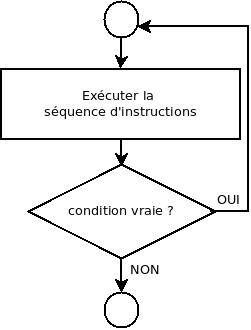
\includegraphics[width=0.8\linewidth,height=0.8\textheight,keepaspectratio=true]{/home/clr/Documents/Cours/DEV1Q2/TDBoucle/fr/image/boucleFaire.jpg}
						\end{center}
                
                    \caption[boucleFaire.jpg]{boucleFaire.jpg}
                \end{figure}
                    
            \par
        Par exemple : 
            \par
        
			
		\subparagraph{Somme de nombres} 
		
					\textcolor{white}{.} \par
				 Apr\`es chaque nombre, on demande \`a l'utilisateur s'il y a encore un nombre \`a additionner.
            \par
        \begin{verbatim}
// Lit des valeurs entières et retourne la somme des valeurs lues.
module sommeNombres() → entier
    encore : booléen // est-ce qu’il reste encore une valeur à additionner ?
    valeur : entier // un des termes de l’addition
    somme : entier // la somme
    somme ← 0
    faire
      lire valeur
      somme ← somme + valeur
      lire encore
    jusqu’à ce que NON encore
    retourner somme
fin module
      \end{verbatim}Avec cette solution, on additionne au moins une valeur.
            \par
        \subsection{pour}
        On va indiquer combien de fois la t\^ache doit \^etre r\'ep\'et\'ee. Cela se fait au travers
        d'une \textbf{variable de contr\^ole} dont la valeur 
        va \'evoluer \textbf{\`a partir d'une valeur de d\'epart jusqu'\`a une valeur finale}.
      
            \par
        En pseudo-code :
            \par
        \begin{verbatim}
pour variable de début à fin [par pas] faire
    séquence d’instructions à exécuter
fin pour
      \end{verbatim} est \'equivalent \`a 
            \par
        \begin{verbatim}
variable ← début
tant que variable ≤ fin faire
    séquence d’instructions à exécuter
    variable ← variable + pas // ou variable ← variable + 1 si le pas est omis.
fin tant que
      \end{verbatim}
        Dans ce type de structure, \verb@début@, 
        \verb@fin@ et \verb@pas@ 
        peuvent \^etre des constantes, des variables ou
        des expressions (le plus souvent \`a valeurs enti\`eres mais on admettra parfois des r\'eels). 
      
            \par
        
        Le \verb@pas@ est facultatif, et g\'en\'eralement omis (dans ce cas, sa valeur par d\'efaut est 1). 
      
            \par
        
        Ce \verb@pas@ est parfois n\'egatif, dans le cas d'un compte \`a rebours, 
        par exemple \,\verb|pour n de 10 à 1 par -1|\,.
      
            \par
        
					\begin{enumerate}
				
			\item 
            Quand le \verb@pas@ est positif, 
            la boucle s'arr\^ete lorsque la \verb@variable@ 
            d\'epasse la valeur de \verb@fin@.
          
			\item 
            Par contre, avec un \verb@pas@ n\'egatif, 
            la boucle s'arr\^ete lorsque la \verb@variable@ 
            prend une valeur plus petite que la valeur de \verb@fin@.
          
					\end{enumerate}
				
            \par
        
        On consid\'erera qu'au cas (\`a \'eviter) o\`u
        
					\begin{enumerate}
				
			\item \verb@début@ est strictement sup\'erieur \`a \verb@fin@ 
            et le \verb@pas@ est positif, la s\'equence d'instructions n'est
            jamais ex\'ecut\'ee (mais ce n'est pas le cas dans tous les langages de programmation !). 
          
			\item 
            Idem si \verb@début@ est strictement inf\'erieur \`a \verb@fin@ 
            mais avec un \verb@pas@ n\'egatif.
          
					\end{enumerate}
				
            \par
        
        Attention de \textbf{ne pas modifier} dans la s\'equence d'instructions une des variables de contr\^ole
        \verb@début@, \verb@fin@ ou \verb@pas@ ! 
      
            \par
        
        Il est aussi fortement \textbf{d\'econseill\'e de modifier \guillemotleft  manuellement }\guillemotright  
        la \verb@variable@ 
        au sein de la boucle \verb@pour@. 
        Il ne faut pas l'initialiser en d\'ebut de boucle, et ne pas s'occuper de sa modification,
         l'instruction \verb@variable ← variable + pas@ \'etant automatique
        et implicite \`a chaque \'etape de la boucle. 
      
            \par
        
        Il est aussi d\'econseill\'e d'utiliser \verb@variable@ \`a la sortie
        de la structure pour sans lui affecter une nouvelle valeur.
      
            \par
        \begin{figure}[hbt]
				    \begin{center}
					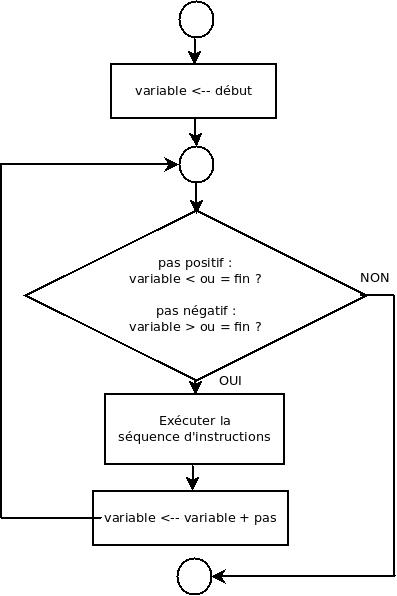
\includegraphics[width=0.8\linewidth,height=0.8\textheight,keepaspectratio=true]{/home/clr/Documents/Cours/DEV1Q2/TDBoucle/fr/image/bouclePour.jpg}
						\end{center}
                
                    \caption[bouclePour.jpg]{bouclePour.jpg}
                \end{figure}
                    
            \par
        Par exemple : 
            \par
        \begin{verbatim}
// Affiche les nombres de 1 à 10.
module compterJusque10 () // version avec pour
    nb : entier
    pour nb de 1 à 10 faire // par défaut le pas est de 1
      afficher nb
    fin pour
fin module
    \end{verbatim}
			
		\subparagraph{Afficher les nombres plus petits que n} 
		
					\textcolor{white}{.} \par
				On affiche uniquement les nombres inf\'erieurs (pas strictement) \`a n.
            \par
        \begin{verbatim}
// Reçoit un nombre et affiche les nombres de 1 à ce nombre.
module afficherN(n↓ : entier)
    nb : entier
    pour nb de 1 à n faire
      afficher nb
    fin pour
fin module
    \end{verbatim}
			
		\subparagraph{Afficher les nombres pairs plus petits que 10} 
		
					\textcolor{white}{.} \par
				On affiche uniquement les nombres pairs jusqu'\`a 10.
            \par
        \begin{verbatim}
// Reçoit un nombre et affiche les nombres pairs jusqu’à ce nombre.
// n : limite des nombres à afficher.
Exemple : si n vaut 10, les nombres pairs de 1 à 10 sont : 2, 4, 6, 8, 10.
module afficherPair (n↓ : entier)
    nb : entier
    pour nb de 2 à n par 2 faire
      afficher nb
    fin pour
fin module
    \end{verbatim}
			
		\subparagraph{Afficher les nombres pairs plus petits que n} 
		
					\textcolor{white}{.} \par
				On affiche uniquement les nombres pairs jusqu'\`a la limite n.
            \par
        \begin{verbatim}
// Reçoit un nombre et affiche les nombres pairs jusqu’à ce nombre.
// n : limite des nombres à afficher.
// Exemple : si n vaut 10, les nombres pairs de 1 à 10 sont : 2, 4, 6, 8, 10.
module afficherPair (n↓ : entier)
    i: entier
    pour i de 1 à n DIV 2 faire
      afficher 2 * i
    fin pour
fin module
    \end{verbatim}
			
		\subparagraph{Afficher n nombres pairs} 
		
					\textcolor{white}{.} \par
				On affiche les n premiers nombres pairs.
            \par
        \begin{verbatim}
// Reçoit un nombre et affiche ce nombre de nombres pairs.
// n: le nombre de nombres à afficher.
// Exemple : si n vaut 10, les 10 premiers nombres pairs sont : 2, 4, 6, 8, 10, 12, 14, 16, 18, 20.
module afficherPair ()
    i : entier
    pour i de 1 à n faire
      afficher 2 * i
    fin pour
fin module
    \end{verbatim}
			
		\subparagraph{Somme de nombres} 
		
					\textcolor{white}{.} \par
				L'utilisateur indique le nombre de termes au d\'epart.
            \par
        \begin{verbatim}
// Lit des valeurs entières et retourne la somme des valeurs lues.
module sommeNombres() → entier
    nbValeurs : entier // nb de valeurs à additionner
    valeur : entier // un des termes de l’addition
    somme : entier // la somme
    i : entier // itérateur
    somme ← 0 // la somme se construit petit à petit. Elle vaut 0 au départ
    lire nbValeurs
    pour i de 1 à nbValeurs faire
      lire valeur
      somme ← somme + valeur
    fin pour
    retourner somme
fin module
    \end{verbatim}\subsection{Quel type de boucle choisir ?}
		    En pratique, il est possible d'utiliser syst\'ematiquement la boucle tant que qui peut s'adapter
        \`a toutes les situations. Cependant, 
        
					\begin{itemize}
				
			\item 
              il est plus clair d'utiliser la boucle \verb@pour@ 
              dans les cas o\`u le nombre d'it\'erations est fix\'e et connu \`a l'avance
              (par l\`a, on veut dire que le nombre d'it\'erations est d\'etermin\'e au moment o\`u on arrive \`a la boucle). 
            
			\item 
              La boucle \verb@faire@ convient quant \`a elle dans les cas o\`u le contenu de la boucle doit \^etre parcouru au moins une fois,
            
			\item 
              alors que dans \verb@tant que@, le nombre de parcours peut \^etre nul si la condition initiale est fausse.
            
					\end{itemize}
				
            \par
        \begin{figure}[hbt]
				    \begin{center}
					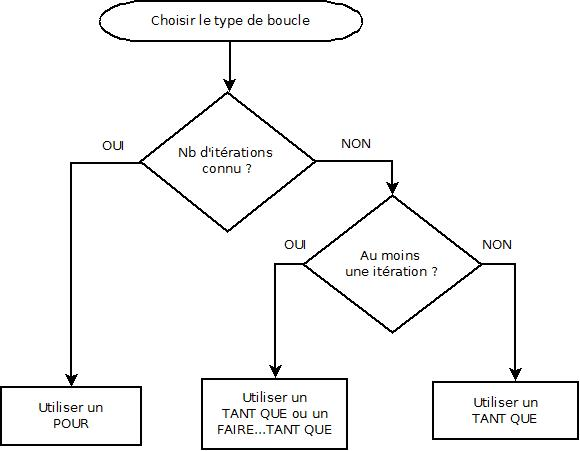
\includegraphics[width=0.8\linewidth,height=0.8\textheight,keepaspectratio=true]{/home/clr/Documents/Cours/DEV1Q2/TDBoucle/fr/image/boucleChoixType.jpg}
						\end{center}
                
                    \caption[boucleChoixType.jpg]{boucleChoixType.jpg}
                \end{figure}
                    
            \par
        \subsection{suite de nombres}
		    Un exemple simple pourrait \^etre celui-ci : 
		    \guillemotleft  \textit{\'Ecrire l'algorithme qui affiche les n premiers
        termes de la suite : 2, 4, 6. . . }\guillemotright 
      
            \par
        
        Puisqu'on doit \'ecrire plusieurs nombres et qu'on sait exactement combien, 
        on se tournera tout naturellement vers une boucle \verb@pour@.
      
            \par
        
        Le cas le plus simple est lorsque le nombre \`a afficher \`a l'\'etape \verb@i@ 
        peut \^etre calcul\'e en fonction de \verb@i@ seulement. L'algorithme est alors
      
            \par
        \begin{verbatim}
pour i de 1 à n faire
    afficher f (i)
fin pour
      \end{verbatim}Par exemple, pour afficher la suite des n premiers nombres pairs
            \par
        \begin{verbatim}
module nombrePair (n↓ : entier)
    i : entier
    pour i de 1 à n faire
      afficher 2 * i
    fin pour
fin module
      \end{verbatim}
        Parfois, il est difficile (voire impossible) de trouver f (i). On suivra alors une autre approche
        qui revient \`a calculer un nombre \`a afficher \`a partir du nombre pr\'ec\'edemment affich\'e (ou, plus
        exactement, de calculer le suivant \`a partir du nombre qu'on vient d'afficher). La structure
        g\'en\'erale est alors
      
            \par
        \begin{verbatim}
nb ← {1re valeur à afficher}
pour i de 1 à n faire
    afficher nb
    nb ← {calculer ici le nb suivant}
fin pour
      \end{verbatim}
        Dans l'exemple de la suite paire, le 1er nombre \`a afficher est 
        2 et le nombre suivant se calcule en ajoutant 2 au nombre courant.
      
            \par
        \begin{verbatim}
module suite1 (n↓ : entier)
    nb, i : entiers
    nb ← 2
    pour i de 1 à n faire
      afficher nb
      nb ← nb + 2
    fin pour
fin module
      \end{verbatim}\subsection{3 pas en avant, 2 pas en arri\`ere}
		    Dans certains cas, il n'est pas possible de d\'eduire directement le nombre suivant en connaissant juste le nombre pr\'ec\'edent. 
		    Prenons un exemple un peu plus compliqu\'e pour l'illustrer.
		    \guillemotleft  \textit{\'Ecrire l'algorithme qui affiche les n premiers termes de la suite : 1, 2, 3, 4, 3, 2, 3, 4, 5, 4, 3. . }. \guillemotright 
      
            \par
        
        Si on vient d'\'ecrire, disons un 3, impossible sans information suppl\'ementaire, de connaitre
        le nombre suivant. Il faudrait savoir si on est en phase d'avancement ou de recul et combien
        de pas il reste \`a faire dans cette direction.
      
            \par
        
        Ajoutons des variables pour retenir l'\verb@état@ o\`u on est.
      
            \par
        \begin{verbatim}
module suite3Avant2Arrière(n↓ : entier)
    nb, nbPasRestants, direction, i : entiers
    nb ← 1
    nbPasRestants ← 3 // 3 pas
    direction ← 1 // en avant
    pour i de 1 à n faire
      afficher nb
      nb ← nb + direction // faire un pas dans la bonne direction
      nbPasRestants ← nbPasRestants - 1
      si nbPasRestants = 0 alors // il est temps de changer de direction
        direction ← -direction
        si direction = 1 alors
          nbPasRestants ← 3
        sinon
          nbPasRestants ← 2
        fin si
      fin si
    fin pour
fin module
      \end{verbatim}
        On obtient un algorithme plus long mais qui respecte toujours le sch\'ema vu.
      
            \par
        
        Un conseil : essayez de respecter ce sch\'ema et vous obtiendrez plus facilement un algorithme
        correct et lisible, \'egalement dans les cas particuliers.
      
            \par
        \section{selon que}Avec ces structures, plusieurs branches d'ex\'ecution sont disponibles. L'ordinateur choisit la
    branche \`a ex\'ecuter en fonction de la valeur d'une variable (ou parfois d'une expression) ou
    de la condition qui est vraie.\subsection{selon que (version avec listes de valeurs)}En pseudo-code :
            \par
        \begin{verbatim}
selon que variable vaut
    liste_1 de valeurs séparées par des virgules :
      // instructions lorsque la valeur de la variable est dans liste_1
    liste_2 de valeurs séparées par des virgules :
      // instructions lorsque la valeur de la variable est dans liste_2
    ...
    liste_n de valeurs séparées par des virgules :
      // instructions lorsque la valeur de la variable est dans liste_n
    autres :
      // instructions lorsque la valeur de la variable
      // ne se trouve dans aucune des listes précédentes
fin selon que
      \end{verbatim}Notez que le cas \verb@autres@ est facultatif.
            \par
        
        Dans ce type de structure, comme pour la structure \verb@si-alors-sinon@, une seule des s\'equences
        d'instructions sera ex\'ecut\'ee. On veillera \`a ne pas faire apparaitre une m\^eme valeur dans
        plusieurs listes. Cette structure est une simplification d'\'ecriture de plusieurs alternatives
        imbriqu\'ees.
      
            \par
        
        Elle est \'equivalente \`a : 
      
            \par
        \begin{verbatim}
si variable = une des valeurs de la liste_1 alors
    // instructions lorsque la valeur est dans liste_1
sinon
    si variable = une des valeurs de la liste_2 alors
      // instructions lorsque la valeur est dans liste_2
    sinon
      ...
      si variable = une des valeurs de la liste_n alors
        // instructions lorsque la valeur est dans liste_n
      sinon
        // instructions lorsque la valeur de la variable
        // ne se trouve dans aucune des listes précédentes
      fin si
    fin si
fin si
      \end{verbatim}
        \'Ecrivons un algorithme qui lit un jour de la semaine sous forme d'un nombre entier (1 pour
        lundi, . . ., 7 pour dimanche) et qui affiche en clair ce jour de la semaine.
      
            \par
        \begin{verbatim}
// Lit un nombre entre 1 et 7 et affiche en clair le jour de la semaine correspondant.
module jourSemaine()
    jour : entier
    lire jour
    selon que jour vaut
      1 : afficher "lundi"
      2 : afficher "mardi"
      3 : afficher "mercredi"
      4 : afficher "jeudi"
      5 : afficher "vendredi"
      6 : afficher "samedi"
      7 : afficher "dimanche"
    fin selon que
fin module
    \end{verbatim}En Java :
            \par
        \begin{verbatim}
switch (variable){
    case val1 :
      // instructions lorsque la valeur de la variable est val1
      break;
    case val2 :
    case val3 :
    case val4 :
      // instructions lorsque la valeur de la variable est val2 ou val3 ou val4
      break;
    ...
    case valN  :
      // instructions lorsque la valeur de la variable est valN
      break;
    default :
      // instructions lorsque la valeur de la variable
      // ne se trouve dans aucune des listes précédentes
}
      \end{verbatim}Notez que le cas \verb@default@ est facultatif.
            \par
        
        Notez le \verb@break@ \`a la fin de chaque (groupe de)\verb@ case@.
      
            \par
        
        La variable peut \^etre de type \verb@byte@, \verb@short@, 
        \verb@char@, \verb@int@\verb@String@ et 
        les types \'enum\'er\'es que nous verrons plus tard.
      
            \par
        
        Elle est \'equivalente \`a : 
      
            \par
        \begin{Java}
if (variable == val1){
      // instructions lorsque la valeur de la variable est val1
} else if (variable ==  val2 || variable ==  val3 || variable == val4){
      // instructions lorsque la valeur de la variable est val2 ou val3 ou val4
} else if (variable == valN){
      // instructions lorsque la valeur de la variable est valN
} else {
      // instructions lorsque la valeur de la variable
      // ne se trouve dans aucune des listes precedentes
}      \end{Java}Par exemple : 
            \par
        \begin{Java}
import java.util.Scanner;
public class Test{
  public static void main(String[] args){
      Scanner clavier = new Scanner(System.in);
      String produit = clavier.next();
      switch(produit) {
        case "Coca" :
        case "Sprite" :
        case "Fanta" :
        prixDistributeur = 60;
        break;
      case "IceTea" :
        prixDistributeur = 70;
        break;
      default :
        prixDistributeur = 0;
        break;
      }
      System.out.println(prixDistributeur);
    }
}
      \end{Java}\subsection{selon que (version avec conditions)}En pseudo-code :
            \par
        \begin{verbatim}
selon que
    condition_1 :
      // instructions lorsque la condition_1 est vraie
    condition_2 :
      // instructions lorsque la condition_2 est vraie
    ...
    condition_n :
      // instructions lorsque la condition_n est vraie
    autres :
      // instructions à exécuter quand aucune
      // des conditions précédentes n’est vérifiée
fin selon que
      \end{verbatim}
        Comme pr\'ec\'edemment, une et une seule des s\'equences d'instructions est ex\'ecut\'ee. On
        veillera \`a ce que les conditions ne se \guillemotleft  recouvrent \guillemotright  pas, c'est-\`a-dire que deux d'entre elles
        ne soient jamais vraies simultan\'ement. 
      
            \par
        C'est \'equivalent \`a : 
            \par
        \begin{verbatim}
si condition_1 alors
    // instructions lorsque la condition_1 est vraie
sinon
    si condition_2 alors
      // instructions lorsque la condition_2 est vraie
    sinon
      ...
      si condition_n alors
        // instructions lorsque la condition_n est vraie
      sinon
        // instructions à exécuter quand aucune
        // des conditions précédentes n’est vérifiée
      fin si
    fin si
fin si
      \end{verbatim}Par exemple : 
            \par
        \begin{verbatim}
// Lit un nombre et affiche si ce nombre est strictement positif , strictement négatif ou nul.
module signeNombre()
    nb : entier
    lire nb
    selon que 
      nb < 0 :
        afficher "le nombre", nb, " est négatif"
      nb > 0 :
        afficher "le nombre", nb, " est positif"
      autres : 
        afficher "le nombre", nb, " est nul"
    fin selon que
fin module
    \end{verbatim}En Java :
            \par
        Il n'existe pas de \verb@switch@ avec condition, 
		  il faut l'\'ecrire comme une succession de \verb@if@.
            \par
        \begin{Java}
if (condition_1){
      // instructions lorsque la condition_1 est vraie
} else if (condition_2){
      // instructions lorsque la condition_2 est vraie
} ... 
} else if (condition_n){
      // instructions lorsque la condition_n est vraie
} else {
      // instructions a executer quand aucune
      // des conditions precedentes n est verifiee
}
      \end{Java}Par exemple : 
            \par
        \begin{Java}
import java. util .Scanner;
public class Test {
    public static void main(String [] args) {
      Scanner clavier = new Scanner(System.in);
      int nb = clavier.nextInt();
      if (nb>0) {
        System.out. println (" positif ");
      } else if (nb==0) {
        System.out. println ("nul");
      } else {
        System.out. println (" negatif ");
      }
    }
}
    \end{Java}\section{Exercices}
				Maintenant, mettons tout \c ca en pratique.
      
            \par
        \subsection{Compr\'ehension d'algorithme}
          Pour ces exercices, nous vous demandons de comprendre des algorithmes donn\'es. 
          
			
		\subparagraph{Compr\'ehension} 
		
                \textcolor{white}{.} \par
            
							  Que vont-ils afficher ?
              
					\begin{itemize}
				
			\item \begin{verbatim}
module boucle1 ()
    x : entier
    x ← 0
    tant que x < 12 faire
      x ← x+2
    fin tant que
    afficher x
fin module
				\end{verbatim} \textcolor{gray}{\underline{\hspace*{2em}}} 
			\item \begin{verbatim}
module exerciceB()
    a,b,c : entier
    lire b,a
    si a > b alors
      c ← a DIV b
    sinon
      c ← b MOD a
    fin si
    afficher c
fin module
				\end{verbatim}Si les nombres lus sont respectivement 2 et 3 ? 
            \par
         \textcolor{gray}{\underline{\hspace*{1em}}} Si les nombres lus sont respectivement 4 et 1 ? 
            \par
         \textcolor{gray}{\underline{\hspace*{1em}}} 
			\item \begin{verbatim}
module exerciceC ()
    x1, x2 : entier
    ok : booléen
    lire x1, x2
    ok ← x1 > x2
    si ok alors
      ok ← ok ET x1 = 4
    sinon
      ok ← ok OU x2 = 3
    fin si
    si ok alors
      x1 ← x1 * 1000
    fin si
    afficher x1 + x2
fin module
				\end{verbatim}Si les nombres lus sont respectivement 2 et 3 ? 
            \par
         \textcolor{gray}{\underline{\hspace*{3em}}} Si les nombres lus sont respectivement 4 et 1 ? 
            \par
         \textcolor{gray}{\underline{\hspace*{3em}}} 
					\end{itemize}
				
            \par
        \subsection{Compr\'ehension de codes Java}
          Pour ces exercices, nous vous demandons de comprendre des codes Java donn\'es. 
          
			
		\subparagraph{Compr\'ehension} 
		
                \textcolor{white}{.} \par
            
							  Que vont-ils afficher si \`a chaque fois les deux nombres lus au d\'epart sont successivement 2, 3 et 4 ?
							
					\begin{itemize}
				
			\item \begin{Java}
import java.util.Scanner;
public class Exercice1 {
    public static void main(String [] args) {
        Scanner clavier = new Scanner(System.in);
        int nb1 = clavier.nextInt();
        int nb2 = clavier.nextInt();
        int nb3 = clavier.nextInt();
        if (nb1 < nb2){
          System.out.print(nb1);
        } else {
          System.out.print(nb2);
        } 
    }
}
        \end{Java} \textcolor{gray}{\underline{\hspace*{1em}}} 
			\item \begin{Java}
import java.util.Scanner;
public class Exercice2 {
    public static void main(String [] args) {
        Scanner clavier = new Scanner(System.in);
        int nb1 = clavier.nextInt();
        int nb2 = clavier.nextInt();
        int nb3 = clavier.nextInt();
        if (nb1 > nb2 && nb1 > nb3){
          System.out.print(nb1);
        } else {
            if (nb2 > nb3){
              System.out.print(nb2);
            } else {
              System.out.print(nb3);
            }
        } 
    }
}
        \end{Java} \textcolor{gray}{\underline{\hspace*{1em}}} 
			\item \begin{Java}
import java.util.Scanner;
public class Exercice3 {
    public static void main(String [] args) {
        Scanner clavier = new Scanner(System.in);
        int nb1 = clavier.nextInt();
        int nb2 = clavier.nextInt();
        int nb3 = clavier.nextInt();
        switch (nb1){
          case 1 : System.out.print("premier"); break;
          case 2 : System.out.print("deuxieme"); break;
          case 3 : System.out.print("troisieme"); break;
          default : System.out.print("pas dans le trio");
        } 
    }
}
        \end{Java} \textcolor{gray}{\underline{\hspace*{10em}}} 
			\item \begin{Java}
import java.util.Scanner;
public class Exercice3 {
    public static void main(String [] args) {
        Scanner clavier = new Scanner(System.in);
        int nb1 = clavier.nextInt();
        int nb2 = clavier.nextInt();
        int nb3 = clavier.nextInt();
        switch (nb1){
          case 1 : System.out.print("premier");
          case 2 : System.out.print("deuxieme");
          case 3 : System.out.print("troisieme");
          default : System.out.print("pas dans le trio");
        } 
    }
}
        \end{Java} \textcolor{gray}{\underline{\hspace*{20em}}} 
					\end{itemize}
				
            \par
        \subsection{\`A vous de jouer...}
          Il est temps de se lancer et d'\'ecrire vos premiers modules et programmes Java correspondant. 
          Voici quelques conseils pour vous guider dans la r\'esolution de tels probl\`emes :
          
					\begin{itemize}
				
			\item il convient d'abord de bien comprendre le probl\`eme pos\'e ; assurez-vous qu'il est parfaitement sp\'ecifi\'e ;
			\item d\'eclarez ensuite les variables (et leur type) qui interviennent dans l'algorithme ; les noms des variables risquant de ne pas \^etre suffisamment explicites ;
			\item \textbf{mettez en \'evidence les variables \guillemotleft  donn\'ees \guillemotright , les variables \guillemotleft  r\'esultats \guillemotright  et les variables de travail ;}
			\item n'h\'esitez pas \`a faire une \'ebauche de r\'esolution en fran\c cais avant d'\'elaborer l'algorithme d\'efinitif pseudo-cod\'e.
			\item \'Ecrivez la partie algorithmique \textbf{AVANT} de vous lancer dans la programmation en Java.
					\end{itemize}
				
            \par
        
        \'Ecrivez les algorithmes et codez les programmes Java correspondant qui 
          
					\begin{enumerate}
				
			\item \'etant donn\'e deux nombres quelconques, recherche et affiche le plus
              grand des deux. Attention ! On ne veut pas savoir si c'est le premier ou le deuxi\`eme qui est
              le plus grand mais bien quelle est cette plus grande valeur. Le probl\`eme est donc bien d\'efini
              m\^eme si les deux nombres sont identiques.
            
			\item \'etant donn\'e trois nombres quelconques, recherche et affiche le plus grand des trois.
			\item affiche un message indiquant si un entier est strictement n\'egatif, nul ou strictement positif.
			\item \'etant donn\'e trois nombres, recherche et affiche si le premier des 
            trois appartient \`a l'intervalle donn\'e par le plus petit et le plus grand des deux autres (bornes exclues). 
            Qu'est-ce qui change si on inclut les bornes ?
			\item \'etant donn\'e une \'equation du deuxi\`eme degr\'e, d\'etermin\'ee par le coefficient de x\texttwosuperior  , le coefficient de x et le terme ind\'ependant, 
            recherche et affiche la (ou les) racine(s) de l'\'equation (ou un message ad\'equat s'il n'existe pas de racine r\'eelle).
			\item \`a partir d'un moment exprim\'e par 2 entiers, heure et minute, affiche le moment qu'il sera une minute plus tard.
			\item v\'erifie si une ann\'ee est bissextile. Pour rappel, les ann\'ees bissextiles sont les ann\'ees multiples de 4.
             Font exception, les multiples de 100 (sauf les multiples de 400 qui sont bien bissextiles). Ainsi 2012 et 2400 sont bissextile mais pas 2010 ni 2100.
					\end{enumerate}
				
            \par
        
			
		\subparagraph{Stationnement alternatif} 
		
					\textcolor{white}{.} \par
				
          Dans une rue o\`u se pratique le stationnement alternatif, du 1 au 15 du mois, on se gare du c\^ot\'e des maisons ayant un num\'ero impair, 
          et le reste du mois, on se gare de l'autre c\^ot\'e.
          \'Ecrivez un algorithme et le code java correspondant qui, sur base de la date du jour et du num\'ero de maison devant laquelle
          vous vous \^etes arr\^et\'e, indique si vous \^etes bien stationn\'e ou non.
        
            \par
        
			
		\subparagraph{La fi\`evre monte} 
		
					\textcolor{white}{.} \par
				
          Chez l'humain la temp\'erature corporelle normale moyenne est de 37 \textdegree C (entre 36,5 \textdegree C et 37,5 \textdegree C selon les individus). 
          La fi\`evre est d\'efinie par une temp\'erature rectale au repos sup\'erieure ou \'egale \`a 38,0 \textdegree C. 
          Une fi\`evre au-del\`a de 40 \textdegree C  est consid\'er\'ee comme un risque de sant\'e majeur et imm\'ediat. 
          Lorsque la fi\`evre est mod\'er\'ee (de 37,7 \textdegree C \`a 37,9 \textdegree C), on parle de f\'ebricule.\par
				
          [Wikipedia]
        
            \par
        
          \'Ecrivez un module fi\`evre qui lit une temp\'erature au clavier et qui affiche si le patient a de la
          temp\'erature (sup\'erieure ou \'egale \`a 38,0\textdegree C) ET si cette cette fi\`evre est mod\'er\'ee (entre 38,0\textdegree C 
          et 40,0\textdegree C) ou \`a risque (strictement sup\'erieur \`a 40,0\textdegree C). 
          Rien ne doit \^etre affich\'e si le patient n'a pas de fi\`evre.
        
            \par
        \'Ecrivez le code java correspondant.
            \par
        
			
		\subparagraph{Taxes communales} 
		
					\textcolor{white}{.} \par
				
          Dans ma commune, les taxes communales des enl\`evements des immondices s'\'el\`event \`a
          
					\begin{itemize}
				
			\item 80€ pour une personne isol\'ee ;
			\item 135€ pour une famille de 2 ou 3 personnes ;
			\item 175€ pour une famille de 4 personnes ou plus.
					\end{itemize}
				
          \'Ecrivez un module qui lit le nombre de personnes composant la famille et qui affiche le prix de la taxe \`a payer.
        
            \par
        \'Ecrivez le code java correspondant.
            \par
        
			
		\subparagraph{Au cin\'ema} 
		
					\textcolor{white}{.} \par
				
          \`A Bruxelles, lors de chaque projection cin\'ematographique, une taxe de 0,5€ est
          pr\'elev\'ee sur le prix du billet de chaque spectateur.
          
					\begin{itemize}
				
			\item \'Ecrivez un module qui lit le nombre de spectateurs et qui affiche le prix de la taxe \`a payer.
			\item \'Ecrivez le code java correspondant.
			\item 
              Si le film projet\'e est un documentaire, aucune taxe n'est pr\'elev\'ee. 
              \'Ecrivez un module qui lit le nombre de spectateurs et un bool\'een (\`a vrai
              si le film est un documentaire et faux sinon) et qui affiche le prix de la taxe
              \`a payer.
            
			\item \'Ecrivez le code java correspondant.
					\end{itemize}
				
            \par
        
				\end{document}
			